\documentclass[12pt]{article}
\usepackage{latexblog}

% ============================================================
% Blog Metadata
% ============================================================
\blogtitle{Vert.X(2)：Vert.x及SpringBoot在CPU密集型应用下的性能测试}
\blogdate{2022-02-18}
\blogtags{Vert.X, 框架, 闲话编程}
\bloglang{zh}
\blogsummary{}

\begin{document}
\makeblogtitle

在\href{https://www.techempower.com}{Web Framework Benchmarks}中测试vert.x比Spring框架性能高上不少，但vert.x这种响应式框架借助异步编程实现，更多的性能体现实际上跟I/O相关。如果一个应用是I/O密集型的那么毫无疑问vert.x性能对于Springboot来说将是碾压式的，那么，对于几乎没有什么I/O操作的CPU密集型应用，vert.x和springboot谁将更胜一筹？

\section{分析}\label{ux5206ux6790}

在实际进行测试之前，首先凭空思考一番。对于CPU密集型的应用，对性能的影响基本上可以忽略I/O模型所带来的加成了，那么更多的是框架本身的架构上。Springboot有一些缺点：

\begin{itemize}
\tightlist
\item
  它是基于Servlet的，也就是一个请求将对应到一个线程；在高并发的情况下，系统创建的线程数是有上限的，而且线程数目越多，反而性能可能大幅降低
\item
  Springboot本身的调用堆栈十分复杂
\end{itemize}

所以推测，即便是对于CPU密集型应用，vert.x仍然具有较为明显的优势，尤其是对于高并发的场景下，Springboot将更早到达极限。

\section{测试准备}\label{ux6d4bux8bd5ux51c6ux5907}

虽然想当然的认为vert.x性能一定会要比Springboot高，但是毕竟没有数据说话，高到底又高多少呢？为此，我设计了一个性能测试，思路是用两种框架分别实现同样的逻辑，然后部署在docker中用jmeter进行测试。

\subsection{API接口实现}\label{apiux63a5ux53e3ux5b9eux73b0}

测试模拟了一个app的元数据管理系统，从内存中根据app id拿到数据，并返回给客户端。

\begin{Shaded}
\begin{Highlighting}[]
\AttributeTok{@GetMapping}\OperatorTok{(}\StringTok{"/api/v1/\{app\}"}\OperatorTok{)}
\KeywordTok{public}\NormalTok{ AppInfo }\FunctionTok{getAppInfoV1}\OperatorTok{(}\AttributeTok{@PathVariable} \BuiltInTok{String}\NormalTok{ app}\OperatorTok{)}
        \KeywordTok{throws}\NormalTok{ JsonProcessingException}\OperatorTok{,}\NormalTok{ InvalidRequestException}\OperatorTok{,}\NormalTok{ AppNotFoundException }\OperatorTok{\{}
    \ControlFlowTok{return}\NormalTok{ service}\OperatorTok{.}\FunctionTok{getAppInfo}\OperatorTok{(}\NormalTok{app}\OperatorTok{);}
\OperatorTok{\}}
\end{Highlighting}
\end{Shaded}

为了增加一些复杂性，又引入了其他几个api，增加了一些小的东西在返回的结果上。

\begin{Shaded}
\begin{Highlighting}[]
\AttributeTok{@GetMapping}\OperatorTok{(}\StringTok{"/api/v2/\{app\}"}\OperatorTok{)}
\KeywordTok{public}\NormalTok{ ResponseEntity}\OperatorTok{\textless{}}\NormalTok{AppInfo}\OperatorTok{\textgreater{}} \FunctionTok{getAppInfoV2}\OperatorTok{(}\AttributeTok{@PathVariable} \BuiltInTok{String}\NormalTok{ app}\OperatorTok{)}
        \KeywordTok{throws}\NormalTok{ InvalidRequestException}\OperatorTok{,}\NormalTok{ AppNotFoundException }\OperatorTok{\{}
\NormalTok{    AppInfo info }\OperatorTok{=}\NormalTok{ service}\OperatorTok{.}\FunctionTok{getAppInfo}\OperatorTok{(}\NormalTok{app}\OperatorTok{);}

    \ControlFlowTok{return}\NormalTok{ ResponseEntity}\OperatorTok{.}\FunctionTok{ok}\OperatorTok{()}
            \OperatorTok{.}\FunctionTok{header}\OperatorTok{(}\StringTok{"Signature"}\OperatorTok{,}\NormalTok{ service}\OperatorTok{.}\FunctionTok{getSign}\OperatorTok{(}\NormalTok{info}\OperatorTok{))}
            \OperatorTok{.}\FunctionTok{body}\OperatorTok{(}\NormalTok{info}\OperatorTok{);}
\OperatorTok{\}}

\AttributeTok{@PostMapping}\OperatorTok{(}\StringTok{"/api/v1/\{app\}"}\OperatorTok{)}
\KeywordTok{public}\NormalTok{ ResponseEntity}\OperatorTok{\textless{}}\NormalTok{AppInfo}\OperatorTok{\textgreater{}} \FunctionTok{getAppInfoV1ByPost}\OperatorTok{(}\AttributeTok{@PathVariable} \BuiltInTok{String}\NormalTok{ app}\OperatorTok{,}
                                                  \AttributeTok{@RequestBody} \BuiltInTok{Request}\NormalTok{ request}\OperatorTok{)}
        \KeywordTok{throws}\NormalTok{ InvalidRequestException}\OperatorTok{,}\NormalTok{ AppNotFoundException }\OperatorTok{\{}
\NormalTok{    AppInfo info }\OperatorTok{=}\NormalTok{ service}\OperatorTok{.}\FunctionTok{getAppInfo}\OperatorTok{(}\NormalTok{app}\OperatorTok{);}

    \ControlFlowTok{return}\NormalTok{ ResponseEntity}\OperatorTok{.}\FunctionTok{ok}\OperatorTok{()}
            \OperatorTok{.}\FunctionTok{header}\OperatorTok{(}\StringTok{"nonce"}\OperatorTok{,}\NormalTok{ request}\OperatorTok{.}\FunctionTok{getNonce}\OperatorTok{())}
            \OperatorTok{.}\FunctionTok{body}\OperatorTok{(}\NormalTok{info}\OperatorTok{);}
\OperatorTok{\}}

\AttributeTok{@PostMapping}\OperatorTok{(}\StringTok{"/api/v2/\{app\}"}\OperatorTok{)}
\KeywordTok{public}\NormalTok{ ResponseEntity}\OperatorTok{\textless{}}\NormalTok{AppInfo}\OperatorTok{\textgreater{}} \FunctionTok{getAppInfoV2ByPost}\OperatorTok{(}\AttributeTok{@PathVariable} \BuiltInTok{String}\NormalTok{ app}\OperatorTok{,}
                                                  \AttributeTok{@RequestBody} \BuiltInTok{Request}\NormalTok{ request}\OperatorTok{)}
        \KeywordTok{throws}\NormalTok{ InvalidRequestException}\OperatorTok{,}\NormalTok{ AppNotFoundException}\OperatorTok{,}\NormalTok{ JsonProcessingException }\OperatorTok{\{}
\NormalTok{    AppInfo info }\OperatorTok{=}\NormalTok{ service}\OperatorTok{.}\FunctionTok{getAppInfo}\OperatorTok{(}\NormalTok{app}\OperatorTok{);}

    \ControlFlowTok{return}\NormalTok{ ResponseEntity}\OperatorTok{.}\FunctionTok{ok}\OperatorTok{()}
            \OperatorTok{.}\FunctionTok{header}\OperatorTok{(}\StringTok{"Signature"}\OperatorTok{,}\NormalTok{ service}\OperatorTok{.}\FunctionTok{getSign}\OperatorTok{(}\NormalTok{info}\OperatorTok{,}\NormalTok{ request}\OperatorTok{.}\FunctionTok{getNonce}\OperatorTok{()))}
            \OperatorTok{.}\FunctionTok{body}\OperatorTok{(}\NormalTok{info}\OperatorTok{);}
\OperatorTok{\}}
\end{Highlighting}
\end{Shaded}

为了使用同样的流程，我们将业务逻辑抽象成了一起，这样vert.x中实现也十分简单：

\begin{Shaded}
\begin{Highlighting}[]
\NormalTok{Router router }\OperatorTok{=}\NormalTok{ Router}\OperatorTok{.}\FunctionTok{router}\OperatorTok{(}\NormalTok{vertx}\OperatorTok{);}
\NormalTok{router}\OperatorTok{.}\FunctionTok{get}\OperatorTok{(}\StringTok{"/api/v1/:app"}\OperatorTok{)}
        \OperatorTok{.}\FunctionTok{handler}\OperatorTok{(}\NormalTok{context }\OperatorTok{{-}\textgreater{}} \OperatorTok{\{}
            \BuiltInTok{String}\NormalTok{ app }\OperatorTok{=}\NormalTok{ context}\OperatorTok{.}\FunctionTok{pathParam}\OperatorTok{(}\StringTok{"app"}\OperatorTok{);}

\NormalTok{            AppInfo info }\OperatorTok{=}\NormalTok{ service}\OperatorTok{.}\FunctionTok{getAppInfo}\OperatorTok{(}\NormalTok{app}\OperatorTok{);}
\NormalTok{            context}\OperatorTok{.}\FunctionTok{json}\OperatorTok{(}\NormalTok{info}\OperatorTok{);}
        \OperatorTok{\}).}\FunctionTok{failureHandler}\OperatorTok{(}\NormalTok{errorHandler}\OperatorTok{);}
\end{Highlighting}
\end{Shaded}

\subsection{Docker部署}\label{dockerux90e8ux7f72}

为了模拟对资源的限制，使用Docker进行部署是一个十分方便的做法，如下我们将springboot和vertx分别部署在同样的配置下：

\begin{Shaded}
\begin{Highlighting}[]
\FunctionTok{version}\KeywordTok{:}\AttributeTok{ }\StringTok{"2.4"}
\FunctionTok{services}\KeywordTok{:}
\AttributeTok{  }\FunctionTok{app{-}springboot}\KeywordTok{:}
\AttributeTok{    }\FunctionTok{build}\KeywordTok{:}
\AttributeTok{      }\FunctionTok{context}\KeywordTok{:}\AttributeTok{ ./springboot}
\AttributeTok{      }\FunctionTok{dockerfile}\KeywordTok{:}\AttributeTok{ ./Dockerfile}
\AttributeTok{    }\FunctionTok{image}\KeywordTok{:}\AttributeTok{ springboot{-}app:latest}
\AttributeTok{    }\FunctionTok{ports}\KeywordTok{:}
\AttributeTok{      }\KeywordTok{{-}}\AttributeTok{ }\StringTok{"8081:8080"}
\AttributeTok{    }\FunctionTok{mem\_limit}\KeywordTok{:}\AttributeTok{ 4096m}
\AttributeTok{    }\FunctionTok{cpus}\KeywordTok{:}\AttributeTok{ }\FloatTok{4.0}
\AttributeTok{  }\FunctionTok{app{-}vertx}\KeywordTok{:}
\AttributeTok{    }\FunctionTok{build}\KeywordTok{:}
\AttributeTok{      }\FunctionTok{context}\KeywordTok{:}\AttributeTok{ ./vertx}
\AttributeTok{      }\FunctionTok{dockerfile}\KeywordTok{:}\AttributeTok{ ./Dockerfile}
\AttributeTok{    }\FunctionTok{image}\KeywordTok{:}\AttributeTok{ vertx{-}app:latest}
\AttributeTok{    }\FunctionTok{ports}\KeywordTok{:}
\AttributeTok{      }\KeywordTok{{-}}\AttributeTok{ }\StringTok{"8082:8080"}
\AttributeTok{    }\FunctionTok{mem\_limit}\KeywordTok{:}\AttributeTok{ 4096m}
\AttributeTok{    }\FunctionTok{cpus}\KeywordTok{:}\AttributeTok{ }\FloatTok{4.0}
\end{Highlighting}
\end{Shaded}

其中，限制内存为4G，CPU为4个单位。由于我们采取了Java11，可以自动感知内存的限制，所以无需单独为java设置内存参数。

\subsection{jmeter测试}\label{jmeterux6d4bux8bd5}

通过jmeter可以很方便的进行压力测试，其思路是，启动多个线程朝目标机器发送请求，并记录结果。

\begin{figure}
\centering
\pandocbounded{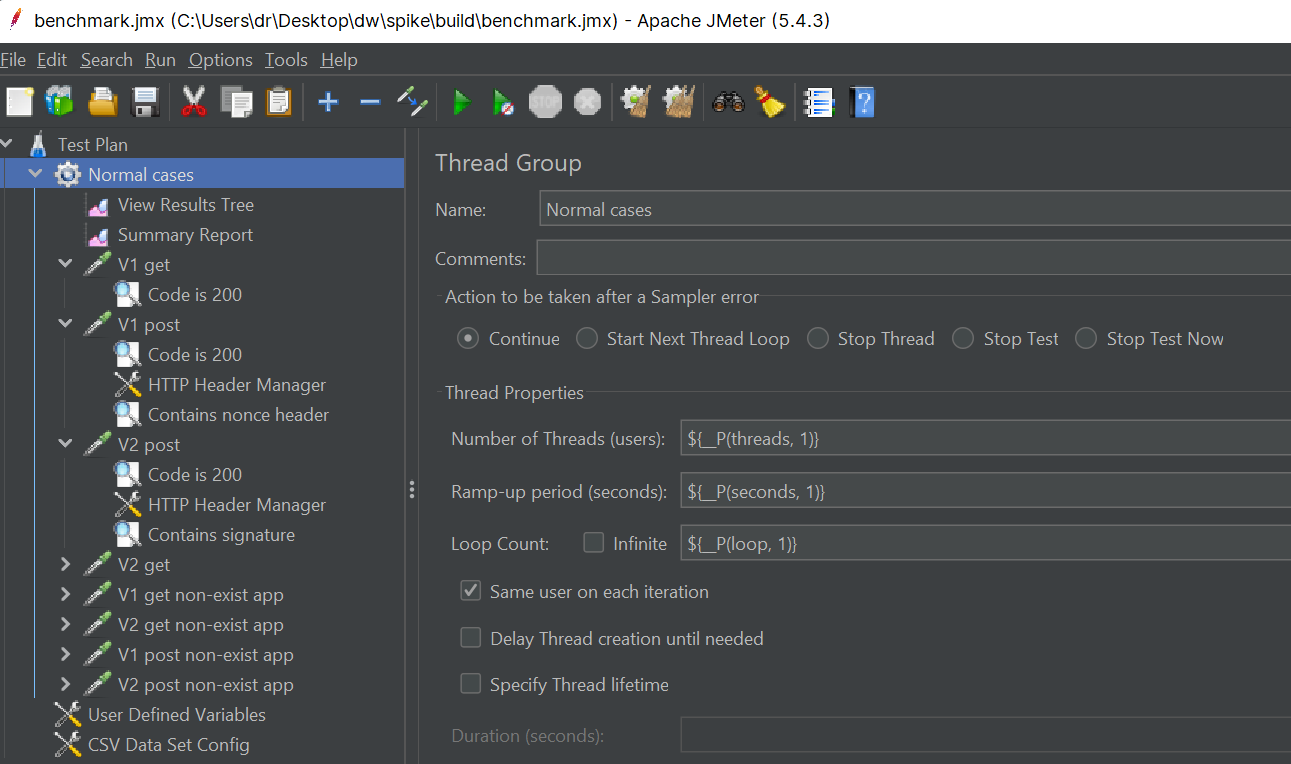
\includegraphics[keepaspectratio,alt={Jmeter配置}]{images/Jmeter-testplan.png}}
\caption{Jmeter配置}
\end{figure}

值得注意的是，

\begin{itemize}
\tightlist
\item
  使用asseration来对结果是否正确进行评估，默认情况下，jmeter根据返回码来判断；但有些场景我们其实是希望它出错的
\item
  使用csv数据源可以方便的将数据均匀化
\item
  使用\texttt{\$\{\_\_P(threads,\ 1)\}}这种形式可以支持将变量从命令行传入
\end{itemize}

最终，我们测试的时候，需要使用命令行（而不是GUI）来进行测试，类似：

\begin{Shaded}
\begin{Highlighting}[]
\ExtensionTok{./apache{-}jmeter{-}5.2.1/bin/jmeter} \AttributeTok{{-}n} \AttributeTok{{-}t}\NormalTok{ benchmark.jmx }\DataTypeTok{\textbackslash{}}
    \AttributeTok{{-}J}\NormalTok{ threads=3000 }\DataTypeTok{\textbackslash{}}
    \AttributeTok{{-}J}\NormalTok{ seconds=0 }\DataTypeTok{\textbackslash{}}
    \AttributeTok{{-}J}\NormalTok{ loop=100 }\DataTypeTok{\textbackslash{}}
    \AttributeTok{{-}l}\NormalTok{ result.jtl }\DataTypeTok{\textbackslash{}}
    \AttributeTok{{-}j}\NormalTok{ result.log}
\end{Highlighting}
\end{Shaded}

\section{测试结果}\label{ux6d4bux8bd5ux7ed3ux679c}

以下是测试的结果:

\pandocbounded{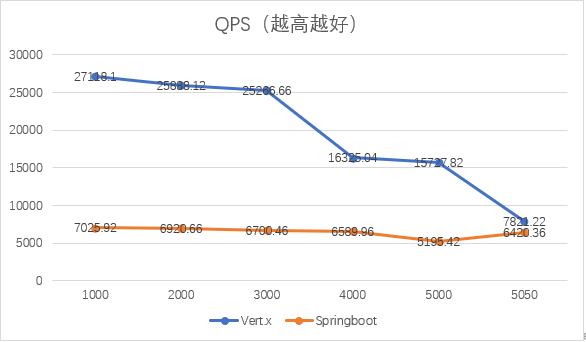
\includegraphics[keepaspectratio]{images/Vertx-qps.png}}

\pandocbounded{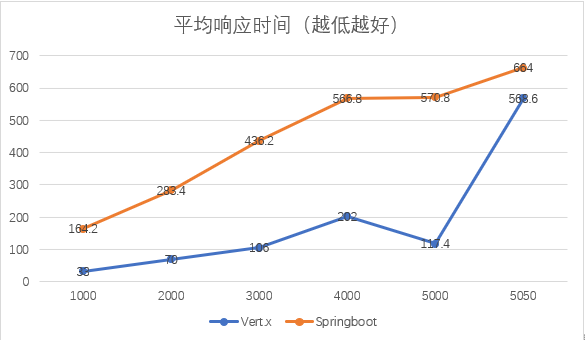
\includegraphics[keepaspectratio]{images/Vertx-rt.png}}

\pandocbounded{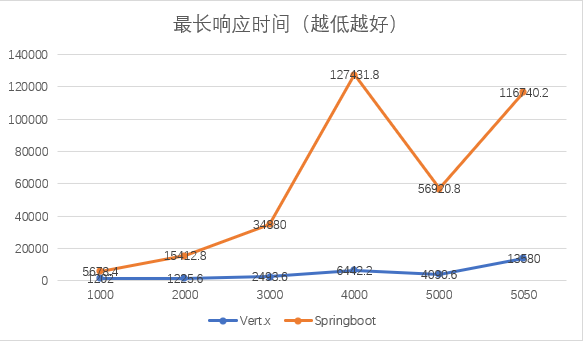
\includegraphics[keepaspectratio]{images/Vertx-mrt.png}}

\pandocbounded{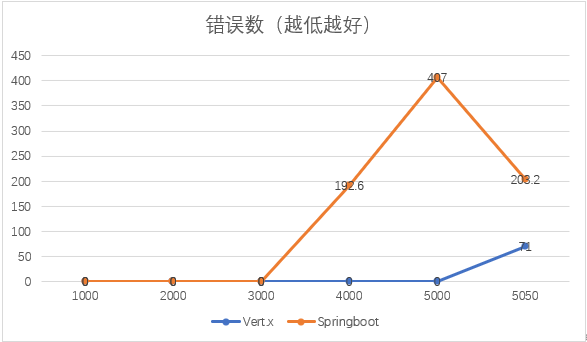
\includegraphics[keepaspectratio]{images/Vertx-err.png}}


\end{document}
